% !TEX encoding = UTF-8 Unicode

\documentclass[twocolumn,10pt,a4j]{jsarticle}
\usepackage{kougai}

\title{小学校教員が利用することを目的としたScratch課題集サイトの制作}
\author{1632075 坂下 駿也 1632093 世戸 \UTF{FA1A}貴   指導教員 須田 宇宙 准教授}
\date{}

\begin{document}
\maketitle

\section{はじめに}

%背景
文部科学省が2020年以降に従来の教育にプログラミング教育を盛り込んだ学習指導要領改定案を発表した.これにより小学校低学年時からプログラミング教育が実施されることになり,児童のプログラミング教育に注目が集まっている.

%問題点
しかし,2020年に向けてプログラミングの授業に関する研修は各々行われているものの,授業を行えるか不安と感じる教職員が多い.実際に,東京都の教職員の85\%はプログラミング授業の実施経験がなく,98\%の教職員が授業の実施に不安を感じている[1].

さらに,ビジュアルプログラミングの解説と例題の提供を同時に行なっているビジュアルプログラミング教材が不足しており,ビジュアルプログラミングを学習した後,教職員は自分で授業用の例題を作成するか,別の教材や問題集などから授業で扱う例題などを引用してくる必要がある.

%目的
そこで本制作では,プログラミング経験及び授業経験のない小学校教員が児童に対して出題する例題を提供することと,それに対する教員の理解を促進することを目的としたプログラミング課題集Webサイトの制作を行うことを目的とする.

\section{小学校のプログラミング教育について}
文部科学省が発表した学習指導要領によると,小学校で行うプログラミング教育は既存の科目にプログラミングを取り入れる形で展開される.実際にビジュアルプログラミングを取り扱うことになるのは,算数での図形の作図,理科での電気の性質の理解,図画工作や音楽の創作,総合的な学習の時間や放課後のクラブ活動等が予想される.しかし2020年に先駆け,既に既存の科目にプログラミングを取り入れている自治体や小学校も少数であるが存在しており,文部科学省がそれらの情報をまとめ,発信するWebサイトも存在している[2].

\section{Webサイトの構成}
本制作は上記のような, 既にプログラミング教育を実践している小学校や教職員を対象としたものではなく,2020 年からプログラミング教育の指導を行うことになる小学校教員を対象にしたプログラミング課題一覧を作成することとし,学年ごとに行われる総合的な学習の時間及び放課後のクラブ活動での使用を想定したものとする.\par
本制作では,「Scratch」を用いて, 文部科学省が提唱した「プログラミング的思考」を構成する「自らの意図を明確化させる思考力」「どのような動きをどのような順序でさせれば良いのかを考える思考力」「どのように組み合わせれば良いかを考える思考力」を育成することを目的とし, 例題を提供することとする. 出題する例題として,「プログラミングの基本的な考え方(順番処理)」を 6 問,「繰り返し処理(ループ)」を 11 問,「条件分岐」を 9 問,「その他(メッセージ)」と応用問題を 3 問ずつ, 計 32 問を作成した. 図1に, 実際の例題提供画面を示す.

\begin{figure}[h]
\begin{center}
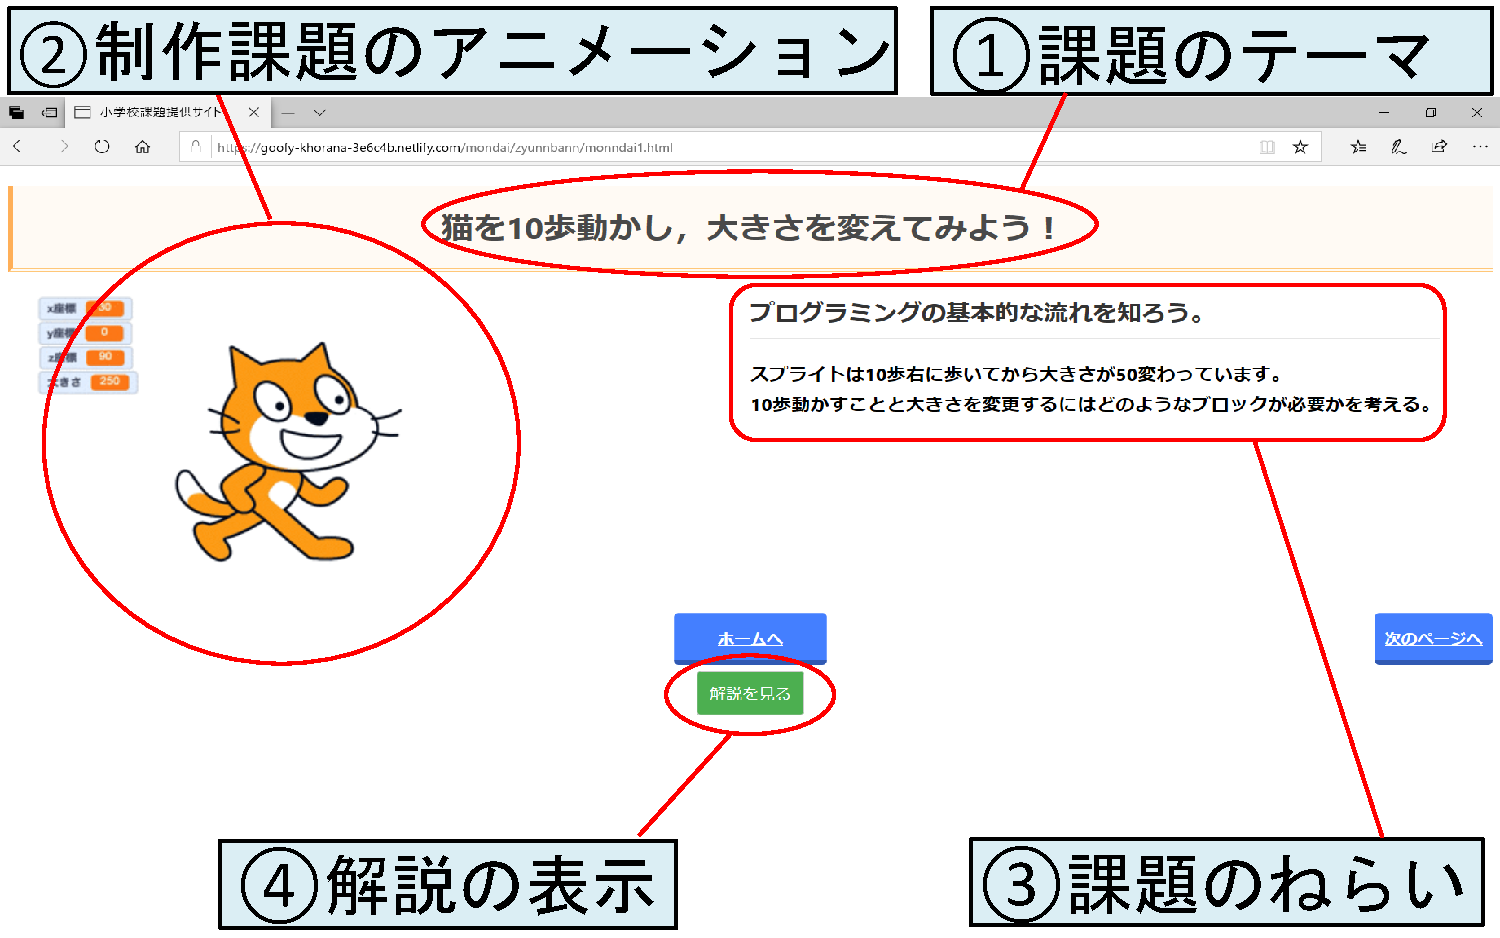
\includegraphics[clip,width=85mm,height=55mm]{zu1.pdf}
\end{center}
\caption{例題の提供画面}
\label{fig:教科書}
\end{figure}

画面上部に\textcircled{\scriptsize 1}その例題で目的とすることを示し,\textcircled{\scriptsize 2}には制作課題のアニメーションをgif画像を用いて表示した. また, \textcircled{\scriptsize 3}には課題のねらいを示し、教員が実際に授業で児童に対しての指導方法を示す.\textcircled{\scriptsize 4}には解答と解説を表示するためのボタンを配置し, このボタンをクリックすることで解答及び解答の解説を確認ができるほか, 問題の解答ファイルのダウンロードも行うことができる. また,「ホームへ」ボタンを押すことでホームページへ,「前のページへ/次のページへ」ボタンを押すことで前後の問題へと移るものとした.

\section{おわりに}
本研究では, 小学校プログラミング教育への導入, プログラミング的思考力を身につける, 教職員のプログラミング教育への知識不足による不安と負担を解消することのできるWebサイトを用いたプログラミング教材を制作した.

\section{参考文献}
\begin{thebibliography}{99}
\bibitem{suda2019} ReseMom: ``小学校のプログラミング教育、先生の98%が「授業の実施に不安」``, \url{https://resemom.jp/article/2019/04/26/50334.html}, 2019/9/01参照
\bibitem{suda2019} 小学校を中心としたプログラミング教育ポータル: ``未来の学びコンソーシアム``, \url{https://miraino-manabi.jp/}, 2019/12/23参照
\end{thebibliography}
\end{document}
